\documentclass{beamer}
\usepackage{mathtools, amsmath, xcolor, graphicx}
\usetheme{Rochester}
\usecolortheme{dolphin}

\author{Joe Bentley and Jake Lane}

\title{Higgs Signal Optimisation}

\institute{}
\subject{Physics}
\date{}
\begin{document}


\frame{\titlepage}


\frame{
\frametitle{Summary}
\begin{enumerate}
\item General background on Higgs
\item How Higgs signals are simulated
\item How the Higgs signal is optimised
\item Problems in optimisation and improvements
\item Possible expansions of the project
\end{enumerate}
}


\frame{
\frametitle{Background}
The Higgs boson is produced in many channels.
\pause
The most common in proton collider experiments is 'gluon gluon Fusion' (ggF)
\begin{figure}
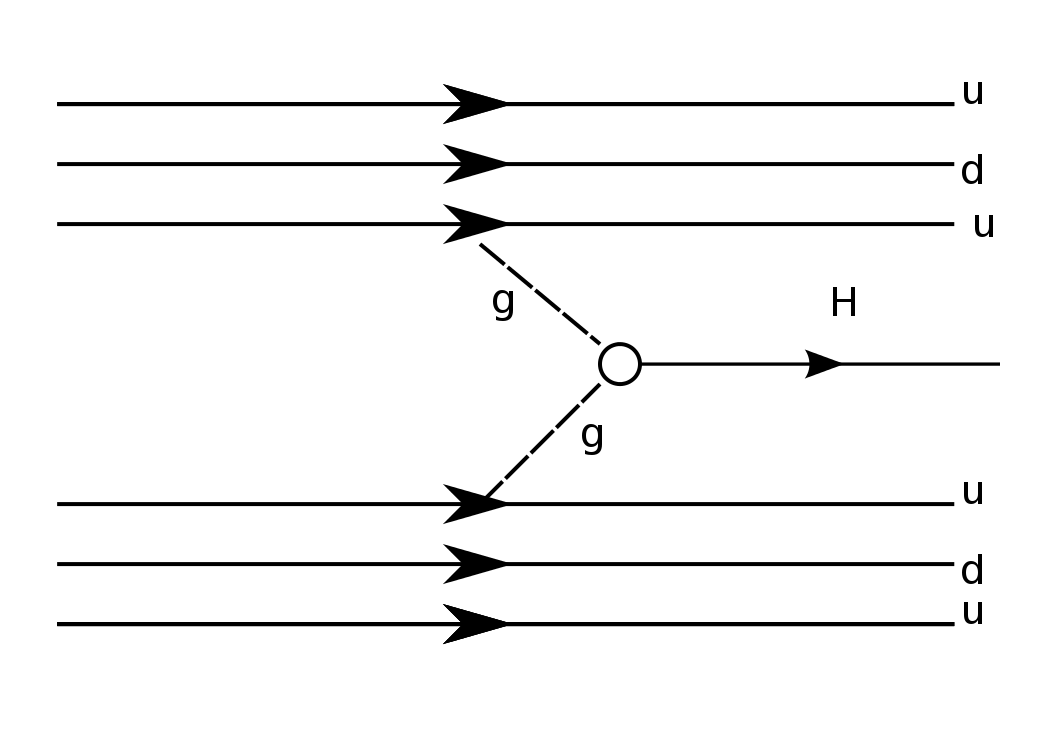
\includegraphics[scale = 0.1]{VBF.png}
\caption{Gluons fusing into a Higgs at a proton-proton interaction}
\end{figure}
\pause
The Higgs decays in a very short period of time in many channels, the most common is 2 bottom quarks, but we investigate the decay into 2 photons (the diphoton channel.)
}

\frame{
\begin{figure}
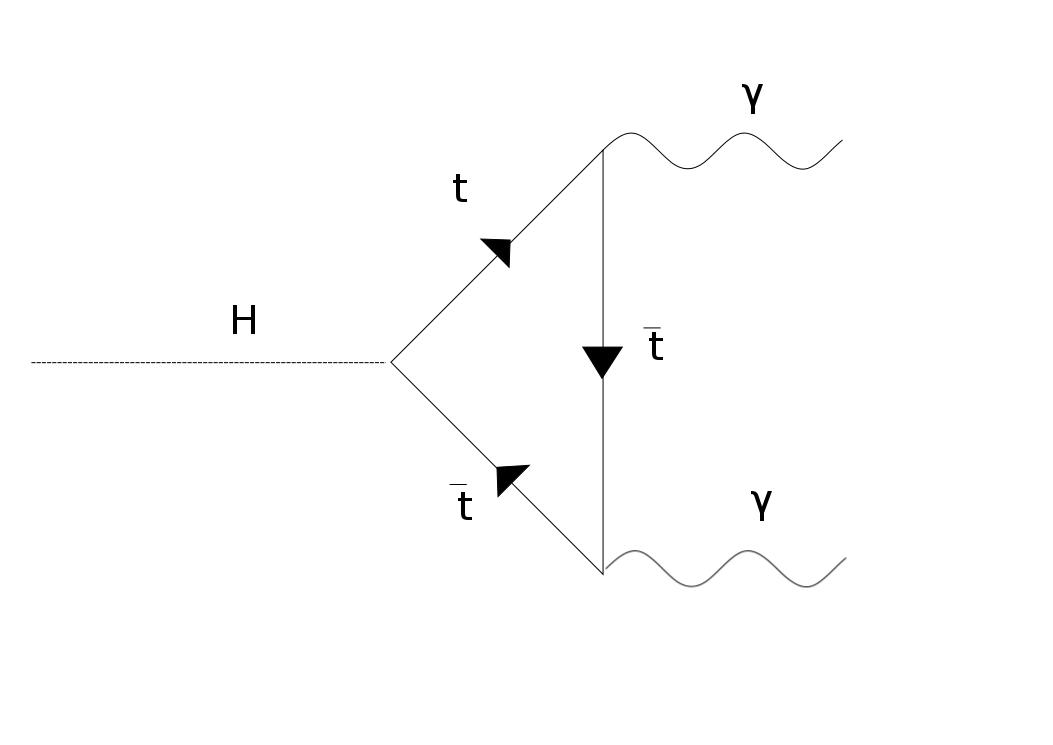
\includegraphics[scale=0.2]{Hyy.png}
\caption{Decay of Higgs into 2 photons}
\end{figure}
This has a branching fraction of order of  $10^{-3}$ but is much  easier to detect experimentally.
}


\frame{
\frametitle{Simulation}

The Higgs events and background events are simulated using PYTHIA. The simulation consists of a text file of the Energy and momentum (4 momentum) of each photon in each event (read collision.) We will use 1 simulation of Higgs events (which still have background in them) and 1 simulation of background events.
}

\frame{
\frametitle{Filter Methods}

\begin{itemize}
  \item There are ~100 Higgs events to ~100,000,000 background events
  \item We need an effective way to distinguish Higgs events from background events
\end{itemize}
}

\frame{
  \frametitle{Filter Methods}

  \begin{enumerate}
    \item Transverse momentum filtering
    \item Pseudorapidity filtering
    \item Azimuthal angle filtering
  \end{enumerate}
}

\frame{
\frametitle{Optimising our Filters}

To optimise our filters so that we have the best ratio of Higgs events to background events, we need to optimise our filter methods for the highest statistical significance $\Sigma$,

\begin{equation}
\Sigma \equiv \frac{S}{\sqrt{S + B}}
\end{equation}

where $S$ is the number of filtered signal events and $B$ is the number of filtered background events.

We apply the filtering and calculate the significance for a series of different parameters, for example for different transverse momenta cuts, to see what gives us the best statistical significance.
}

\frame{
\begin{figure}
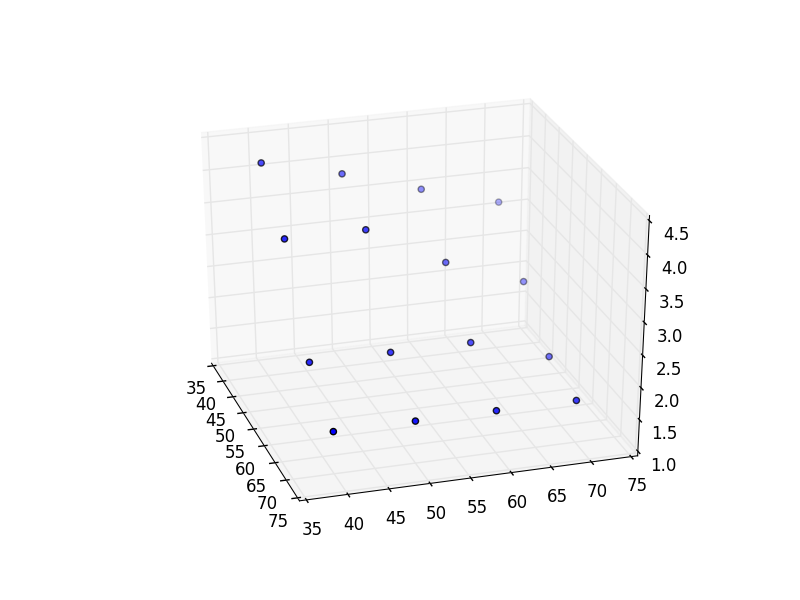
\includegraphics[scale=0.2]{significance1}
\caption{Statistical significance (height of points) for a series of different transverse momenta}
\end{figure}

From graphs like these we can narrow down the ranges of transverse momenta that we filter until we get the highest statistical significance.
}


\end{document}
